\chapter{ Spread of Zika Virus on a Small World Network }

The deterministic models discussed in the chapters above assume that all individuals have an equally small probability of being infected. In this section we build a model for the propagation of Zika virus based on a small world network.

Traditional models of infectious disease dynamics have a long, successful history of describing and modelling infectious disease spread of many diseases. They are quite simple and tractable \citep{fu2013propagation}.

There are certain specific and common situations when the structure of social connectivity is at least as important as the  activity of the underlying infectious agents for the study of transmission of infection and control. This is one among the major reasons that has motivated the modelling of infectious diseases on social networks \cite{fu2013propagation}.



\section{ Vector Borne Disease Propagation on a Small World Network}

In this section we transform a vector borne transmission dynamics of Zika virus to a small world network. As a way of simplifying our model we move from a human-vector-human propagation to a human-human disease propagation.The interaction between mosquitoes and humans become the edges that connect human to human.

We assume that there is a lattice with two layers. One for mosquitoes and the other for human beings. We assume that mosquitoes are stationary and that people have close and remote links. That is mosquitoes do not cover long distances, but just hover around a specific location.
On the other hand, people can travel to distant locations. Close links refer to individual's close acquaintances while distant links refer to and individuals random acquaintances.
 
A mosquito $M_1$ bites a Zika infected person $h_1$ with probability $\alpha_1$. Then transmits the virus to person $h_2$, with a probability of $\alpha_2$. Thus, person $h_1$ is connected to  person $h_2$ through $M_1$. It can then be said that $h_2$ can be infected by $h_1$ with probability $p_1$. Assuming that $\alpha_1 $ and $\alpha_2$ are independent  $p_1 =  \alpha_1 \alpha_2$. 

 If person $h_3$ travels to the place where $h_1$ lives or gets close enough that he gets bitten by mosquito $M_1$ can be infected probability $\alpha_3$. Thus, $\alpha_3$ is the probability that person $h_3$ travels and get bitten by mosquito $M_1$. It can be said that $h_1$ infects $h_3$ with probability $p_2$, because $h_1$ is connected to $h_3$ through $M_1$. Assuming $\alpha_1$ and $\alpha_3$ are independent, $p_2 = \alpha_1 \alpha_3$.
\begin{figure}[h!]
\centering
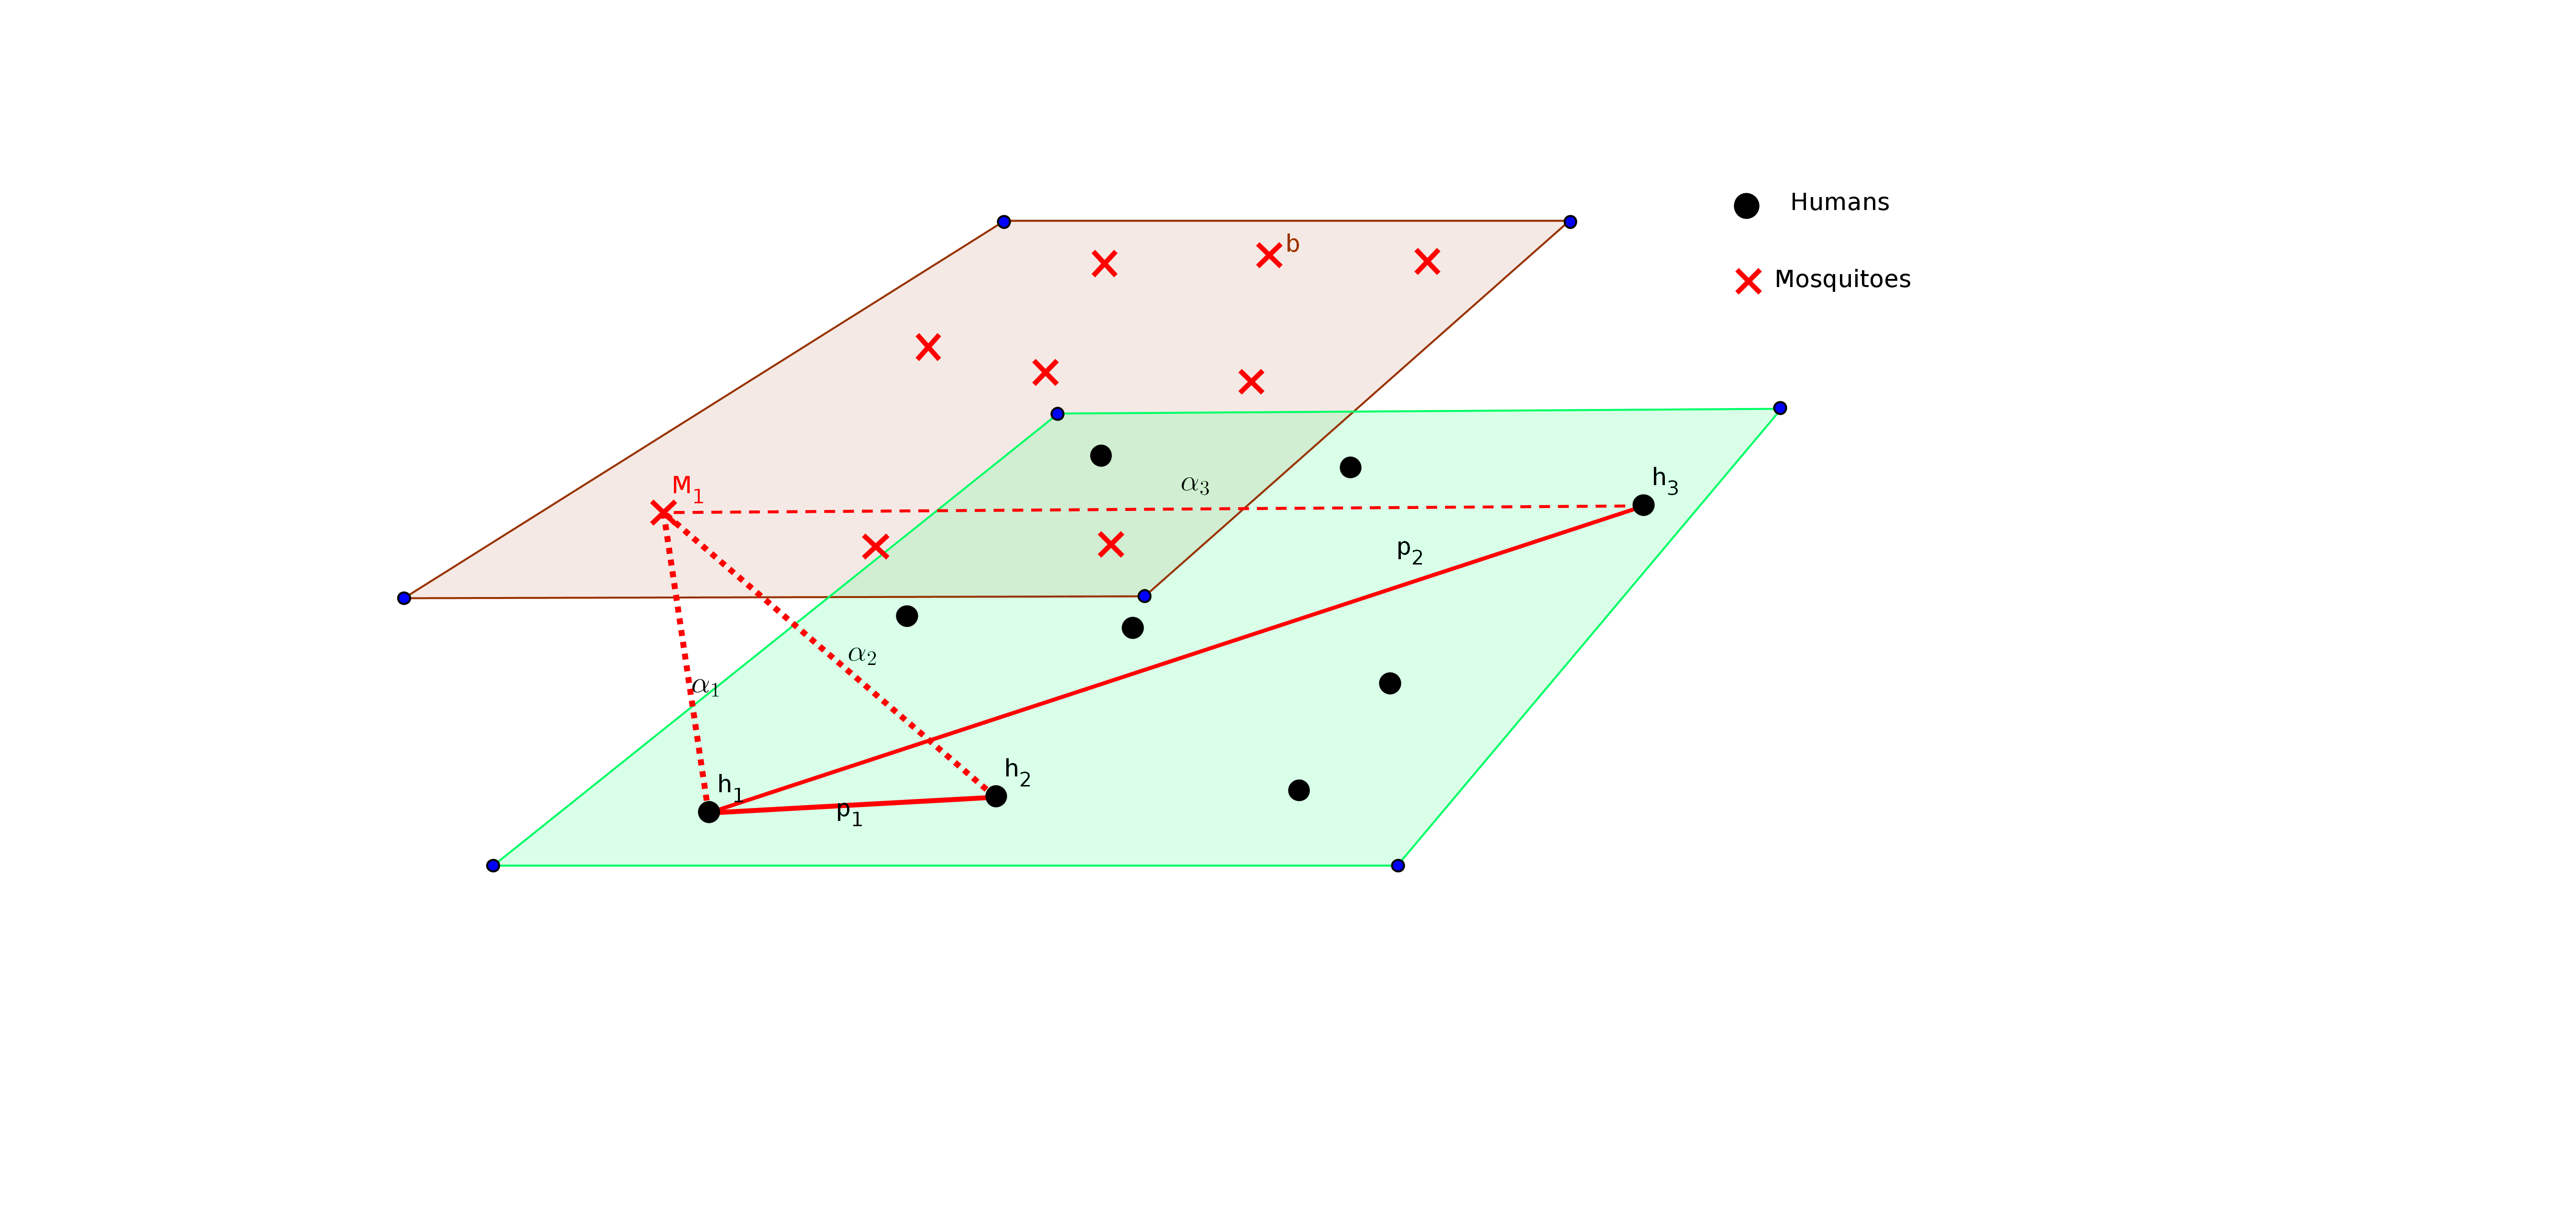
\includegraphics[scale=1]{images/human_mosquito.png}
\caption{Disease transmission through a vector} \label{fig5}
\end{figure}
The phenomenon of infecting a close like  or distant link can be expressed in 4 cases.


\begin{itemize}
\item[i).] $h_2$ may get infected by $h_1$ through $M_1$. In this case $h_1$ and $h_2$ are referred to as near neighbours.
\item[ii).] $h_4$ may travel to a place close enough to get the infection from $h_1$ through $M_1$. In this case $h_3$  referred to as a distant neighbour.
\item[iii).] $ h_1$ may travel to a place close enough to infect $h_4$  through another mosquito in that vicinity.In this case $h_3$ is  referred to as a distant neighbour.
\item[iv).] $h_1$  and $h_3$ may both travel to some place at the same time and $h_1$ transmits the infection to $h_3$ and this case is neglected. Thus, in the this case $h_1$ and $h_3$ would not be referred to as near or distant neighbours.
\end{itemize}

The probabilities of cases (ii) and (iii)
might be different but we assume that we can average them out and   use single value for $p_2$. We neglect probability in case (iv), since we consider it to be small compared to case (ii) and case(iii). We assume that the population of mosquitoes is homogeneous and that they bite humans uniformly and randomly.

The existence of near and distant neighbours in the disease infection dynamics of Zika virus on a lattice with two layers in \ref{fig5} makes it possible to represent the dynamics of disease spread on a small world network in figure \ref{fig 5.2}. Thus, in modelling the spread of Zika virus on a small world network, the dynamics of transmission through mosquitoes are represented by the edges of the graph. An edge is drawn between two vertices, whenever there is a likelihood of transmission from one to another via a mosquito bite as can be seen in figure \ref{fig5}.

\begin{figure}[h!]
\begin{minipage}[c]{1\textwidth}
 \centering
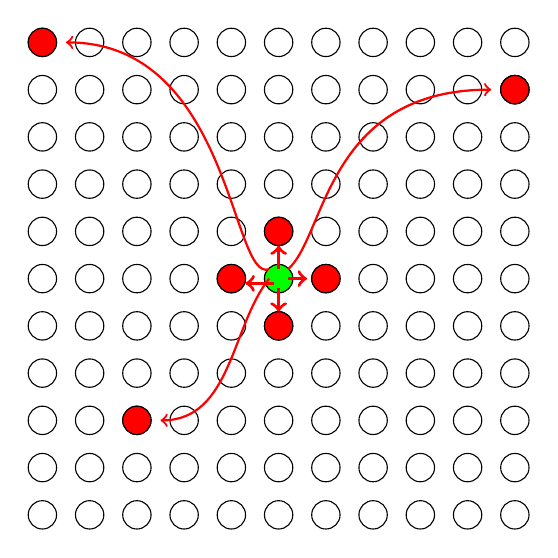
\begin{tikzpicture}[scale=0.6]
  \foreach \x in {0,...,10}
        \foreach \y in {0,...,10}
        {
        \draw (\x,\y) circle (0.3cm);
        }

\filldraw[fill=green!, draw=black](5,5) circle (0.3cm);
\filldraw[fill=red!, draw=black](2,2) circle (0.3cm);
\filldraw[fill=red!, draw=black](10,9) circle (0.3cm);
\filldraw[fill=red!, draw=black](10,9) circle (0.3cm);
\filldraw[fill=red!, draw=black](4,5) circle (0.3cm);
\filldraw[fill=red!, draw=black](5,4) circle (0.3cm);
\filldraw[fill=red!, draw=black](6,5) circle (0.3cm);
\filldraw[fill=red!, draw=black](5,6) circle (0.3cm);
\filldraw[fill=red!, draw=black](0,10) circle (0.3cm);

\draw[draw=red!,
preaction={->,thick,draw =red!}
] (5.2,5.2) ..controls(6,5.9) and (6,9) ..(9.5,9);
\draw[ draw =red!,thick, ->] (4.8,5.2) .. controls (4,4.9) and (4,10) ..(0.5,10);
\draw[ draw =red!,thick, ->] (4.8,5) .. controls (4,4) and (4,2) ..(2.5,2);
\draw[ draw =red!,very thick, ->] (5.2,5) -- (5.6,5);
\draw[ draw =red!,very thick, ->] (5,5.2) --(5,5.7);
\draw[ draw =red!,very thick, ->] (4.9,4.9) -- (4.3,4.9);
\draw[ draw =red!,very thick, ->] (5,4.8) --(5,4.3);
\end{tikzpicture}
%\caption{Smallworld network structure} \label{fig 5.1}
\end{minipage}
\caption{Smallworld network structure} \label{fig 5.1}
\end{figure}
\section{Small World Methodology}
Having built a small world structure to depict the spread of Zika virus. We now describe the small world methodology of the spread of Zika virus and use it build a model for the transmission of Zika virus.

We  can now suppose that the population is arranged on a regular
2-dimensional square grid.  Where each vertex can infect its 4 nearest neighbours and a number of distant neighbours. Near neighbours in this case refers to individuals that one spends most of their time with, could be colleagues at work or school or people in the same house and distant neighbours refers to random individuals that one is likely to transmit the infection to. 
 
 \begin{figure}[h]
 \centering
 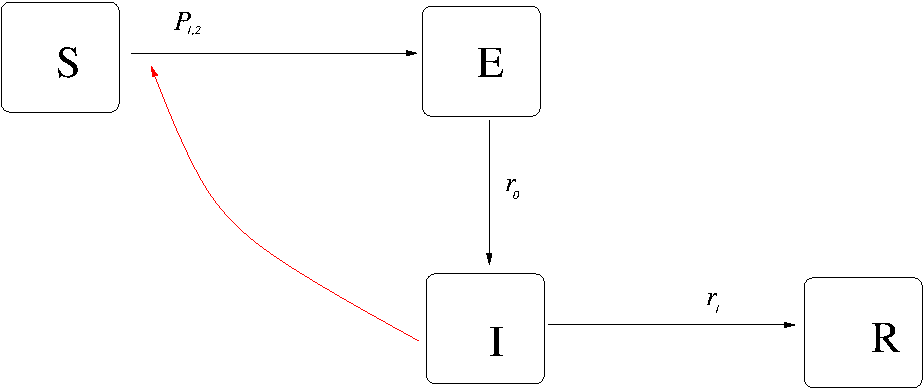
\includegraphics[scale=0.5]{images/swseir.png}
 \caption{State transition diagram} \label{fig 5.2}
\end{figure}

 
Figure \ref{fig 5.1} shows the arrangement of nodes in a small world network and figure \ref{fig 5.2} shows the transmission state diagram. The probabilities of transition from one compartment to another are per day and each day we assume that the given transition occur independently. Transition from :S to E
occurs
with infection probabilities $p_ {1,2} $ based on the small world network structure and: E to I with probability $r_0$ and I to R with probability $r_1$. In figure \ref{fig 5.1}, the infected green node may infect its four near neighbours, with probability $p_1$ and its three remote neighbours with probability $p_2$. By infection we mean transition from susceptible to exposed state. 

Infected individuals can cause susceptible individuals, whom they are linked to, to become exposed with with probability $p_1$ or $p_2$. Infected individuals can  infect their close neighbours with  probability $p_1$ and infect their distant neighbours with probability $p_2$. $p_1 $ and $p_2$ are probabilities of infection per day. Exposed individuals become infected with probability $r_0$ and infected individuals recover with probability $r_1$.

The number of near neighbours $n_1 = 4$ or less, taking into account the boundary cases and number of distant neighbours $n_2$  for each node is independent and  identically distributed. That is for each node $u$ there are $n_2^ {(u)}$ distant neighbours. $n_2^ {(u)} $ is chosen to follow a discrete exponentially decaying distribution 
\begin{equation} 
 \Pr[n_2^{(u)} = k] = c \cdot e^{-\mu k  } \label{5.2.1}
 \end{equation}
 where $c \approx \dfrac{1}{1- e^{-\mu }}$ and $\mu >0$ \citep{fu2013propagation}.
 The degree distribution in most social networks is exponential because of the celebrity effect \citep{estrada2015first}. In social networks, there are few people who have a high number of connections and many others with a few number of connections. In modelling infectious diseases these individuals are referred to as super spreaders.

 The transition probability $r_0$, the number of days an individual is in the exposed state is as a result of a series of Bernoulli trials with mean $\frac{1}{r_0}$, follows a geometric distribution $f_X (x) = (1-r_0) ^ {x-1} r_0$.

 Similarly the infectious period follows a geometric distribution with mean $\dfrac{1}{r_1}$ \citep{fu2013propagation}.

\section{Model}
The model has 6 parameters, they are $N, p_1, p_2, n_2, r_0$ and $r_1$. We let $N$ be the population size of a city or country and is arranged in a regular grid of side length $l $ such that $l^2 = N$. The rest of the parameters have been described above.

A thorough review of literature in \cite{lessler2016times} indicates that the incubation or latent period for Zika virus infection is $11.2$ days after infection, with a $95 \%$ confidence interval of $7.6 -18$. Further the center for disease control and prevention (CDC)
\Jnote{Capitalize CDC name properly.}
indicate that the incubation period for the Zika virus ranges from 3 days to 14 days from infection \citep{krow2017estimated}. Therefore we estimate $r_o$ with $\frac{1}{11.2}$
  
    $95\%$ of the of Zika patients will still have detectable virus infectiousness 18.9 days after infection with a confidence interval of 13.6 -79.4 \citep{lessler2016times}.The infectiousness in Zika infection ends 1.5 - 2 days before the virus becomes undetectable \citep{funk2016comparative}. Thus the chosen value of the infectious period is $18.9 - 1.5 = 17.4$ days. Therefore $r_1$ is estimated to be $\dfrac{1}{17.4}$.

  Hence, we have $\mu$, $p_1$ and $p_2$  as free parameters. Without active control, the average number of secondary infections resulting from a primary  Zika  virus infectious is between 3 and 6. Therefore, we choose 4.5 as the $R_0$. $R_0$ is average number of secondary infections resulting from each new infection.
  
  Since the number of remote neighbours is random and fixed for each, we define $E (n^ {(u)} _2) = \widehat{n_2}$. From the equation \ref{5.2.1}, with $\mu = 0.12$ we obtain $E (n^ {(u)} _2) \approx 8$. We therefore estimate $n_2$ to by the mean $8$.
  
  In this state each infectious individual will infect on average $n_1kp_1 + E[n^{(u)}_2]p_2 $ new individuals everyday. Where k is the average number of near neighbours' links that support possible infection since 
  near neighbours are arranged in clusters, therefore $0.5 \leq k \leq 1$. In our computation we will use $k=0.5$.
    The average number  of individuals infected each day can be estimated by the number of secondary infections an infected individual cause each day, throughout the period they are infectious.

  Thus ;
\begin{align}
n_1k p_1 + \widehat{n_2} p_2 &\approx \dfrac{R_0}{r_1} 
\\ n_1k p_1 + \widehat{n_2} p_2 &\approx 0.2586 \label{eqn 5.32}
\end{align}
thus, 
$p_1 \approx   0.1293- 0.5 \widehat{n_2} p_2$ , in terms of small world parameters $\widehat{n_2}$ and $p_2$.

Now $n_1$ and $n_2$ represent the number of interactions an individual has each day. Hence the  $n_1 + n_2$ is the lower bound is a lower bound of the number of active acquaintances because it is a number of links that are sufficiently intimate to support transmission of the virus. In reality some links would be closer than others and more likely to lead to transmission. We assume that all $n_1$ links are infected with probability $p_1$ and $n_2$ with probability $p_2$ each day. The probabilities $p_1$ and $p_2$ are not necessarily  the same.

Note that the choice of $n_1$ and $n_2$ is not critical; what is more important is the infection probability $n_1kp_1 + n_2p_1$.

We can summarize the parameters of the models as;
\begin{align}
n_1 &= 4 \\
\widehat{n}_2 &= 8 \\
r_0 &= \dfrac{1}{11.2} \approx 0.089 \\
r_1 &= \dfrac{1}{17.4} \approx 0.057 \\
p_1 &= 0.1293 - 4 p_2 \label{eqn 5.1.7}
\end{align}
Now we have one free parameter $p_2$. We can now estimate the number of new infections by;
\begin{align}
E(- \Delta S) = (n_1 k p_1 + \widehat{n}_2    p_2 - r_1) I \label{5.18}
\end{align}

 From equation \ref{5.18} we can estimate the number of new infections as;
\begin{align}
E(- \Delta S) = (2 p_1 + 8 p_2 - 0.057) I  \label{5.1.9}
\end{align}
 
From equation \ref{eqn 5.32}, it can be shown that $p_1$ and $p_2$ have natural bounds. That is taking $p_2 = 0$, implies that $p_1 \leq 0.1293$ . For $p_1 = 0$, we get $p_2 \leq 0.03232$.

Further, from the analysis of the stability of the difference equation of the SEIR compartmental from the largest eigenvalue value, we obtain  the rate of spread of infection is given by ;
\begin{equation}
1- \dfrac{r_o + r_1}{2} + \sqrt{\dfrac{1}{4}(r_o - r_1)^2 + n_k r_o} \label{eqn 5.3.10},
\end{equation}
where as before $n_k = n_1kp_1 + \widehat{n}_2 p_2$ \citep{fu2013propagation}.
From equations \ref{5.18}, it can be seen that the disease will be contained if $n_k < r_1$. If $n_k < r_1$ there will be a negative the increase in the number of infected individuals thus, the disease will be contained. When the probability of recovery is greater than the probability of infection. Individuals will recover before they can infect others, this will result in the out break being contained.

\section{Simulation}
To investigate how disease propagation varies depending on $p_1, p_2, $ and $r_1$ we ran a couple of simulations on a small work network. The code for the simulation is attached in the appendix. 

We initiate the model with one infected individual and an $r_1$ which is relatively small .We simulated our models with various parameters and observe they dynamics  of the infection. 

We ran simulations for 5 cases;
\begin{enumerate}
\item $p_1 = 0.129$ , $p_2 =0$ and $r_1 = 1/17.4$
\item $p_1 = p_2 = 0.02580$ and $r_1 = 1/17.4$ 
\item $p_1 =0 $,$p_2 = 0.0323$ and $r_1 = 1/17.4$
\item $p_1 = 0.0693$ ,$p_2 = 0.0173$ and $r_1 = 1/17.4$
\item $p_1 = 0.045$ ,$p_2 = 0.01125$ and $r_1 = 1/50$
\end{enumerate}

In the first  and third cases we investigate the boundary cases, when$p_1 = 0$ and  $p_2 = 0$ respectively.  In the second case we investigate a case where $p_1 = p_2$. In the    fourth case we investigate and intermediate, where $p_1$ is greater than $p_2$. Lastly we investigate the case where we increase the infectious rate from the initial 17.4 days to 50 days and look at the intermediate case where $p_1 > p_2$. 

\newpage
\section{Results}

\Jnote{Make clear that you are comparing your simulation to determinstic SEIR.
  Also, what are your parameters for SEIR? Shouldn't they be the same
for the first four cases?}

From our simulated model for the transmission dynamics of Zika virus the following results were obtained. In figure \ref{pics:res} we depict the evolution of infected individuals at 20 day intervals in all the cases starting from day 60 to day 120 of the infection.

\textbf{Case 1}

It can be observed that the increase in the number of infected individuals overtime is stochastic in figure \ref{a1}.  From figure \ref{a1} it be seen that the outbreak takes a long time before it dies off. When $p_0$ it implies that the spread of the infection is local. In the first row  of figure \ref{pics:res}, at different time steps infected nodes can be seen in clumps. There are few infections in the first 80 days of the infection as can be seen  in figure \ref{pics:res}, this implies that the infection does not spread rapidly when the spread is only via local links. In figure \ref{a2}, we observe that there few infected and exposed individuals over time. There is a steady decrease in the number of susceptibles and a gradual increase in the number of individuals recovering over time.

\Jnote{Comment on the fact that in our model it's not really an epidemic
  (look at y axes).}

\begin{figure}[h!]
    \centering
    \begin{subfigure}[b]{0.45\textwidth}
        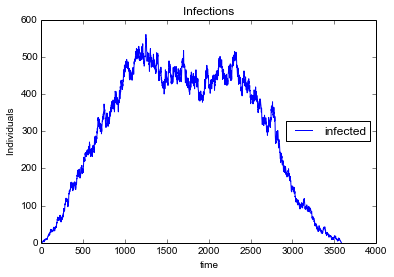
\includegraphics[width=\textwidth]{images/1infections}
        \caption{ progression of infections over time}
        \label{a1}
    \end{subfigure}
     \begin{subfigure}[b]{0.45\textwidth}
        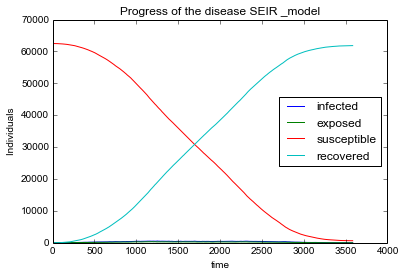
\includegraphics[width=\textwidth]{images/1SEIRmodel}
        \caption{ Flow of individuals in compartments of the infection over time}
        \label{a2}
    \end{subfigure}
  \caption{Infection dynamics for $p_1 = 0.129$, $p=0$ and $r_1 = 1/17.4$ }
\end{figure}

\textbf{Case 2}

In this case we observe that the number of infected individuals over time increases sharply and when it reaches the peaks decreases sharply as can be seen in figure \ref{a21}. In this case there are  both local and distant transmissions of the infections. From \ref{a21} the infection takes a short time to reach its peak and to die off. A lot of people are infected throughout the course of the infection. In figure \ref{a22} we see that number of susceptible individuals decreases slowly up to some point then decrease sharply. The infection does not die out completely, but the epidemic does. Despite there still being individuals who are infected, they cannot spread the virus further as everyone else has developed immunity against it. In the second row of figure \ref{pics:res}, a few clumps can be seen and some random  infections on different days of the infection, representing local transmission and distant transmissions respectively.

\begin{figure}[h!]
    \centering
    \begin{subfigure}[b]{0.45\textwidth}
        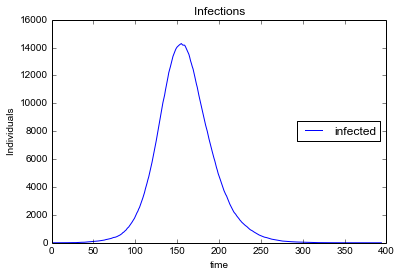
\includegraphics[width=\textwidth]{images/3infections}
        \caption{ Infections over time}
        \label{a21}
    \end{subfigure}
     \begin{subfigure}[b]{0.45\textwidth}
        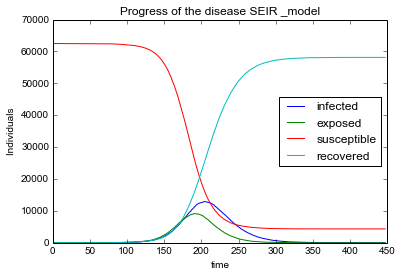
\includegraphics[width=\textwidth]{images/3SEIR}
        \caption{ Flow of individuals in compartments of the infection over time}
        \label{a22}
    \end{subfigure}
  \caption{Infection dynamics for  $p_1 = p_2 = 0.02586$ and $r_1 = 1/17.4$}
\end{figure}
 

 
\textbf{Case 3}

In this case the spread will only be through distant links. The infection will increase sharply, but not as much as in case 2 and will have a lower peak than in case 2 as can be seen in figure \ref{a31}. In figure \ref{a32}, it can be observed that the number of susceptible individuals decreases gradually for a time then decrease sharply. Similar to case 2, the number of infected individuals does not drop to zero. Thus, the curve for susceptible will not go to zero. Some individuals will still be infected, but because most people will develop immunity hence there will no longer be spread of the infection. In the third row of figure \ref{pics:res}, we can observe that on each day of the infection, there are spatially uncorrelated infectious because there are no local infections.

\begin{figure}[h!]
    \centering
    \begin{subfigure}[b]{0.45\textwidth}
        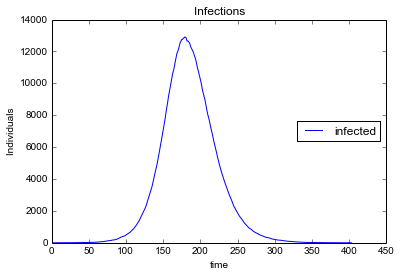
\includegraphics[width=\textwidth]{images/2infections}
        \caption{Progression of the infection overtime}
        \label{a31}
    \end{subfigure}
     \begin{subfigure}[b]{0.5\textwidth}
        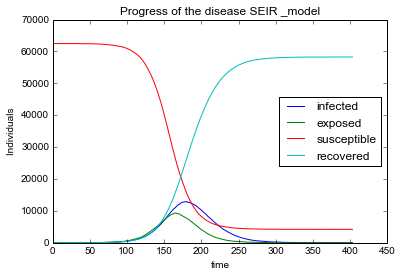
\includegraphics[width=\textwidth]{images/2SEIRmodel}
        \caption{  Flow of individuals in compartments of the infection over time}
        \label{a32}
    \end{subfigure}
  \caption{Infection dynamics for $p_1 = 0$, $p_2=0.0323$ and $r_1 = 1/17.4$}
 \end{figure}
 

\newpage
\begin{minipage}{\linewidth}

\centering
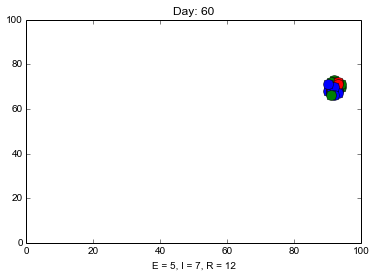
\includegraphics[scale=0.28]{images/1t60.png} \quad
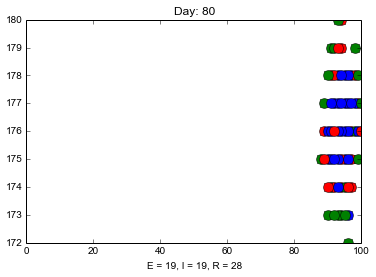
\includegraphics[scale=0.28]{images/1t80.png} \quad
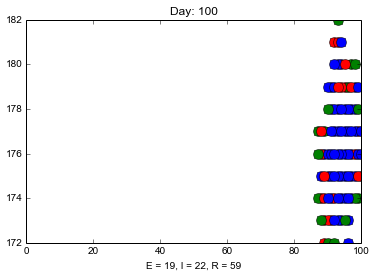
\includegraphics[scale=0.28]{images/1t100.png} \quad
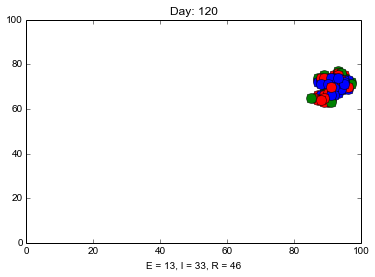
\includegraphics[scale=0.28]{images/1t120.png} 

\medskip
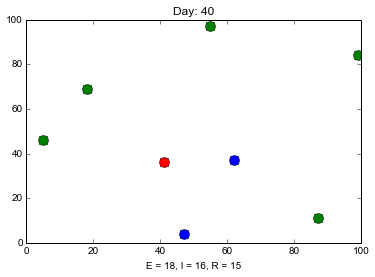
\includegraphics[scale=0.28]{images/2t40.png} \quad
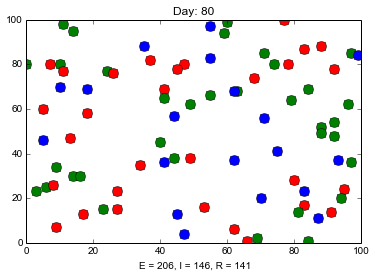
\includegraphics[scale=0.28]{images/2t80.png} \quad
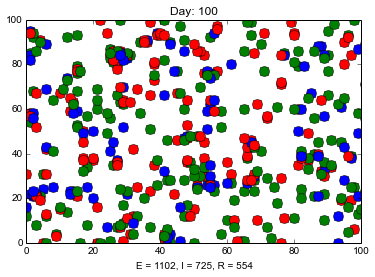
\includegraphics[scale=0.28]{images/2t100.png} \quad
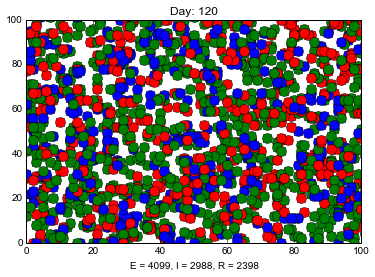
\includegraphics[scale=0.28]{images/2t120.png} 

\medskip
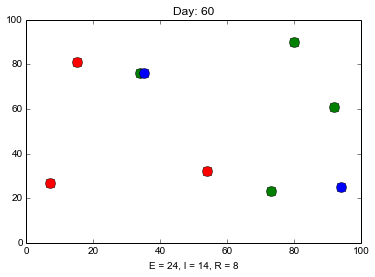
\includegraphics[scale=0.28]{images/3t60.png} \quad
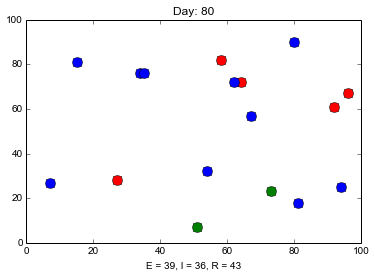
\includegraphics[scale=0.28]{images/3t80.png} \quad
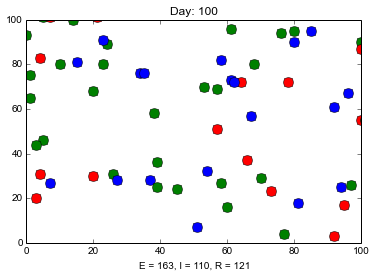
\includegraphics[scale=0.28]{images/3t100.png} \quad
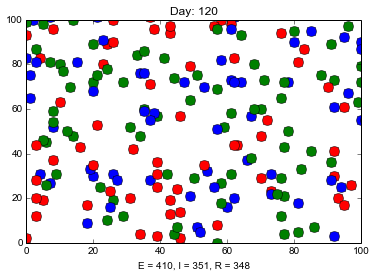
\includegraphics[scale=0.28]{images/3t120.png} 


\medskip
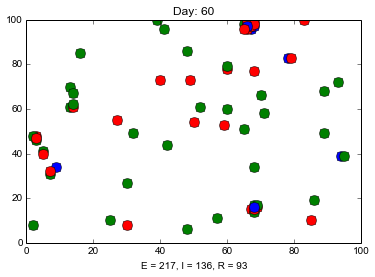
\includegraphics[scale=0.28]{images/4t60.png} \quad
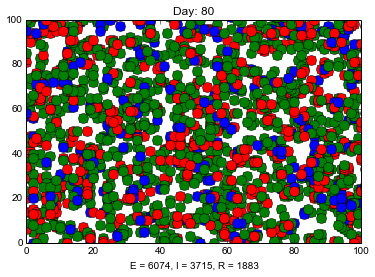
\includegraphics[scale=0.28]{images/4t80.png} \quad
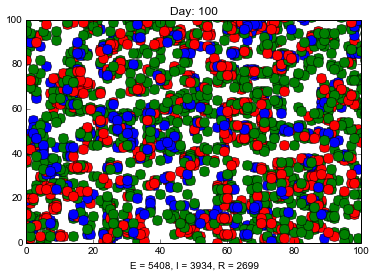
\includegraphics[scale=0.28]{images/4t100.png} \quad
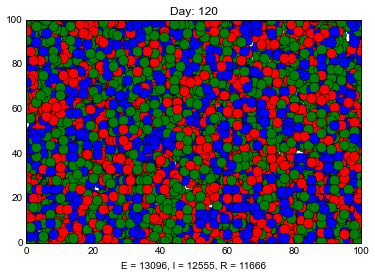
\includegraphics[scale=0.28]{images/4t120.png} 

\medskip
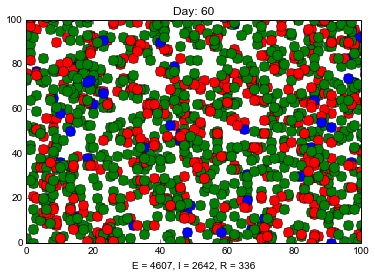
\includegraphics[scale=0.28]{images/5t60.png} \quad
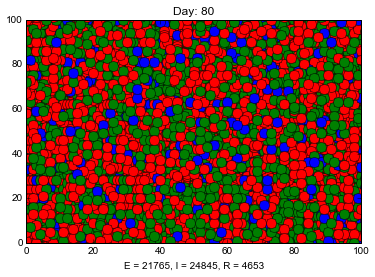
\includegraphics[scale=0.28]{images/5t80.png} \quad
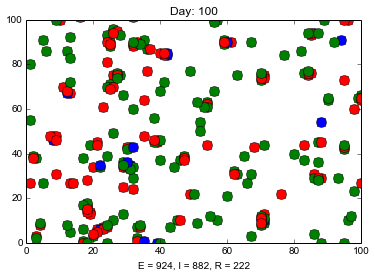
\includegraphics[scale=0.28]{images/5t100.png} \quad
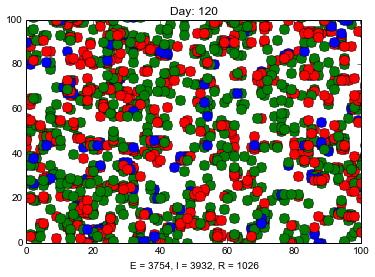
\includegraphics[scale=0.28]{images/5t120.png} 

\captionof{figure}{Each row depicts the evolution at 20 days interval of infection. Infected nodes are shown in red, exposed nodes in blue and recovered nodes in green.}
\label{pics:res}
\end{minipage}

\Jnote{Please check again your code. From the figure in the top row
  it is clear that close links work only left-right.
  Also case 4 looks suspicious to me, though I'm not sure about that.}

\textbf{Case 4}
In this case infection spreads across all links. The probability of of infecting distant neighbour is lower than that of infecting near neighbours. The infection in this case spread similar to cases 2 and 3, though the peak number of infected will be lager than in both cases. Comparing to cases 1 to 3 the infection reaches its peak in a shorter period of time than in the other model figure \ref{a41}. In the figure \ref{a42} the dynamics of the infection is similar to case 3. In the fourth row of figure \ref{pics:res}, we can observe that the infection  in this case will burst early than in all other cases.

\begin{figure}[h!]
    \centering
    \begin{subfigure}[b]{0.45\textwidth}
        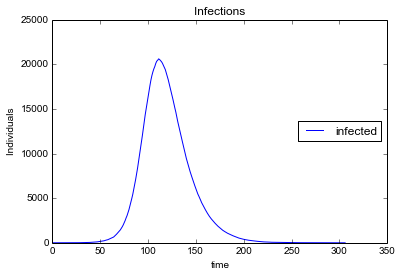
\includegraphics[width=\textwidth]{images/4infections}
        \caption{Progression of infection overtime}
        \label{a41}
    \end{subfigure}
     \begin{subfigure}[b]{0.45\textwidth}
        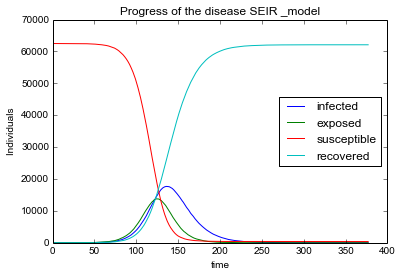
\includegraphics[width=\textwidth]{images/4SEIR}
        \caption{  Flow of individuals in compartments of the infection over time}
        \label{a42}
    \end{subfigure}
  \caption{Infection dynamics for $p_1 = 0.0693 $, $p_2=0.01173$ and $r_1 = 1/17.4$ }
 \end{figure}
 \newpage
 \textbf{Case 5}
 
 In all the previous cases we kept $r_1 = 1/17.4$, were $17.4$ is the number of days an individual is infectious. Since  $r_1$ has larger confidence interval \citep{lessler2016times}, we try  $r_1 = 1/50$.  In this case the infection grows slowly in the early days, but later increases rapidly in a short period of time. In figure \ref{a51} it can be observed that the   number of individuals infected overtime grows exponentially in a short period of time before it starts decreasing. In figure \ref{a52} it can be observed that the number of susceptibles falls drastically because of the rapid spread of the infection.  

\begin{figure}[h!]
    \centering
    \begin{subfigure}[b]{0.45\textwidth}
        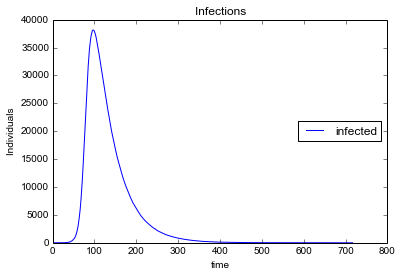
\includegraphics[width=\textwidth]{images/5infections}
        \caption{Progression of infections over time. }
        \label{a51}
    \end{subfigure}
     \begin{subfigure}[b]{0.45\textwidth}
        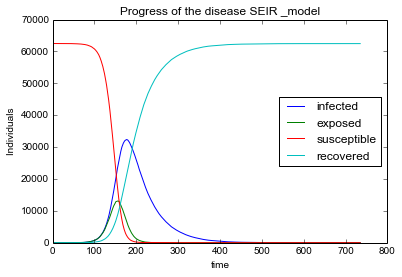
\includegraphics[width=\textwidth]{images/5SEIR}
        \caption{  Flow of individuals in compartments of the infection over time}
        \label{a52}
    \end{subfigure}
  \caption{Infection dynamics for $p_1 = 0.045 $, $p_2=0.01125$ and $r_1 = 1/50$ }
 \end{figure}

 From the first four cases, we can observe that the infections along the distant links  (small world parameters), have a significant effect on the spread of the infection. In case 1 where $p_2 =0$ the infection does not spread rapidly compared to case 3 , where $p_1 =0$. The spread of the infection when $p_1 =p_2$ is quite similar to the spread to case 3 when there are only infections across distant neighbours. The infection spread the faster in case 4 in relation to cases 1 to 3. 
 In case 5, when the infectious period is increased the infection will spread slowly foe some time the later it will explored and spread rapidly because infected individuals will infect more people before they recover.

\section{Conclusion}

In conclusion from our model it can be said that the small world phenomenon, could have  contributed  greatly to the spread of Zika virus across the world. Small world networks can be used to understand why infectious diseases that start in a particular place or area are able to spread all over the world, in a short period of time. With  the increase in people's mobility, there is need to raise awareness on transmission of various infectious diseases in order to reduce the probability of disease transmission across distant
neighbours as well as preventing local infections. 

In coming up with intervention measures, medical specialists might want  to put up measures that reduce the infectious period of Zika patients, that is increasing $r_1$.  Improved health care is one the factors that can lead to  a higher $r_1$. 

The major limitation of this research is the unavailability of time series data on Zika infections, on which the model can be fit and the parameters of the model tested.

In this study we modelled the spread of Zika virus by assuming that an individual has four near neighbours. We would suggest as an area for future research to increase the number of near neighbours.
That is changing the structure of the network. Another area for further research would be, comparing the spread of Zika virus on a random network model with the smallworld model. Further we would suggest modelling the spread of Zika virus by taking into account seasonality. That is building a model where the probabilities of infecting near and distant neighbours depends on the season.

\Jnote{Please give it another pass for typos and grammar.}